\documentclass[11pt]{beamer}
\usepackage[utf8]{inputenc}
\usepackage[T1]{fontenc}
\usepackage{amsmath}
\usepackage{amsfonts}
\usepackage{amssymb}

\usetheme{default}
\usepackage{graphicx}


\setbeamertemplate{footline}
{
    \leavevmode%
    \hbox{%
%        \begin{beamercolorbox}[wd=.4\paperwidth,ht=2.25ex,dp=1ex,center]{author in head/foot}%
%            \usebeamerfont{author in head/foot}\insertshortauthor
%        \end{beamercolorbox}%
        \begin{beamercolorbox}[wd=1\paperwidth,ht=2.25ex,dp=1ex,center]{title in head/foot}%
%            \usebeamerfont{title in head/foot}\insertshorttitle\hspace*{3em}
            \flushright{\insertframenumber{} / \inserttotalframenumber\hspace*{1ex}}%\hspace*{1ex}
    \end{beamercolorbox}}%
    \vskip0pt%
}

\begin{document}
    \author{A. Zelenaya \inst{1}, M. Zelenyi \inst{1,2}, A.A.Turinge \inst{1},  V.G. Nedorezov \inst{1}}
    \title{Chemical composition analysis for X-ray transport container scans. }
    %\subtitle{}
    % \logo{}
    \institute[INR]{
        \inst{1} Institute for Nuclear Research RAS \and
        \inst{2} Moscow Institute of Physics and Technology (SU)
    }
    \date{October 10, 2018}
%    \subject{Moscow}
    \setbeamercovered{transparent}
    \setbeamertemplate{navigation symbols}{}
    \frame[plain]{\maketitle}
    
    \begin{frame}
        \frametitle{Introduction}
            \begin{columns}
            \begin{column}{0.6\textwidth}
                \begin{itemize}
                    \item It is important for national security to control the movement of dangerous or strategically cargo.
                    \item This control can be provided by scanning transport containers by gamma rays produced by bremsstrahlung.
                    \item In this report we consider:
                        \begin{itemize}
                            \item Methodology, existing solution and our proposing method;
                            \item GEANT4 simulation of gamma rays scanning;
                            \item Measurement resolution of gamma rays detector.
                        \end{itemize}
                   
                \end{itemize}
            \end{column}
            \begin{column}{0.4\textwidth} 
        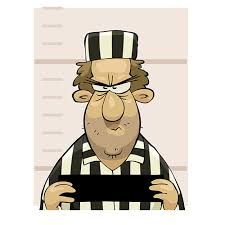
\includegraphics[width=1\textwidth]{figures/terrorist.jpg}
            \end{column}
        \end{columns}  
    \end{frame}
    \begin{frame}
    \frametitle{Methodology: Gamma ray attenuation}
    \begin{columns}
        \begin{column}{0.7\textwidth}
            $$
            T(E_0, t, Z) = \frac{\int \limits_0^{E_0} S(E_0, E) \exp(-\mu(E,Z)\times t)~dE)}{\int \limits_0^{E_0} S(E_0, E)~dE}
            $$
%            \hline
            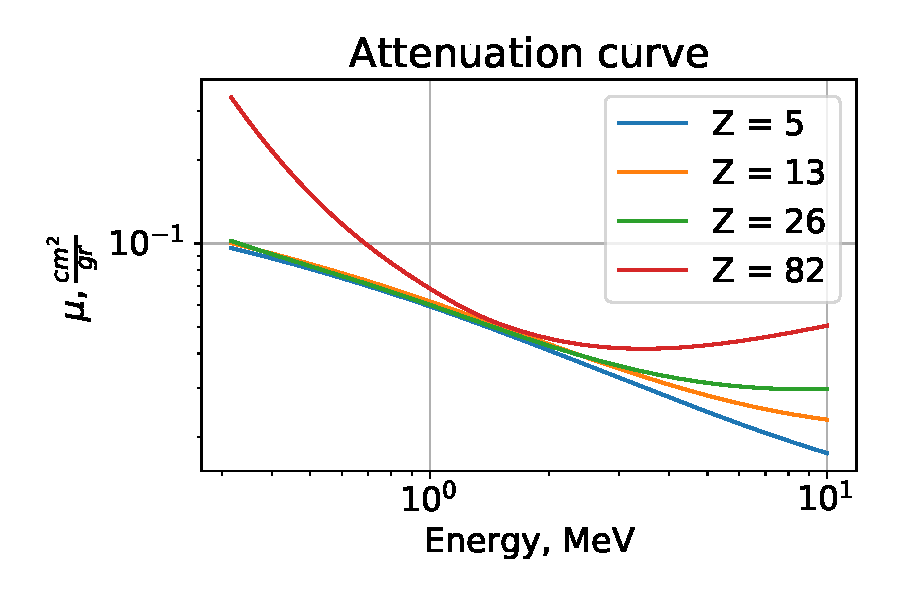
\includegraphics[width=1\textwidth]{figures/Attenuation.pdf}
        \end{column}
    \vline~
        \begin{column}{0.4\textwidth} 
            $T$ -  transmittance\\
            $S(E_0, E)$ - response function\\
            $\mu(E,Z)$ - attenuation\\
            $t$ -  optical thickness\\
            $E_0$ -  up-limit energy of bremsstrahlung\\
            $E$ - energy of gamma ray\\
            $Z$ - charge of nuclei 
%            \hline
            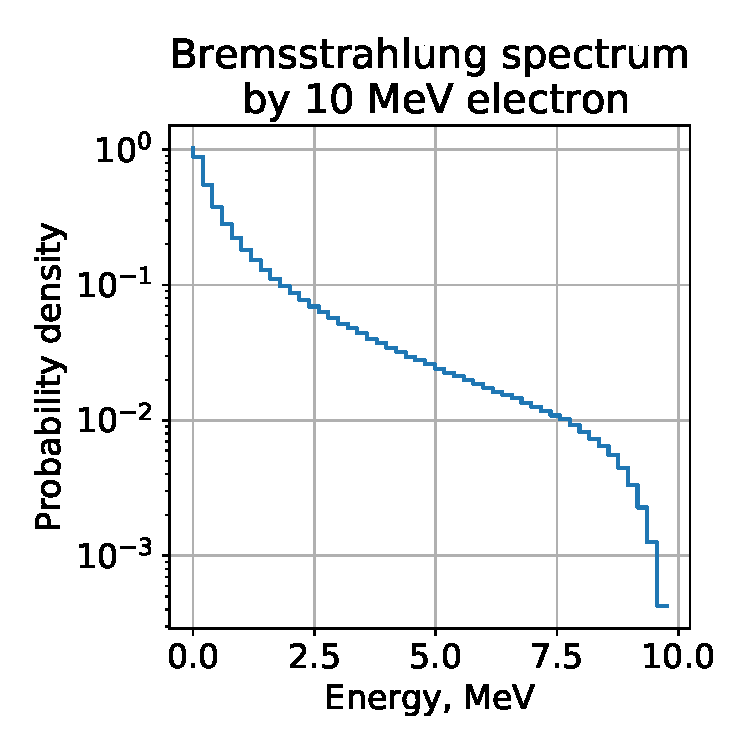
\includegraphics[width=1\textwidth]{figures/Bremsstrahlung.pdf}
        \end{column}
    \end{columns}  
\end{frame}

\begin{frame}
    \frametitle{Methodology: Existing solution}
    \begin{block}{Dual energy method}%<1>
        \begin{itemize}
            \item We can't defined Z if optical thickness $t$ is unknown.
            \item But we can use two electron beams with different energy which give gamma rays with up-limit energy $E^{(1)}_0$ and $E^{(2)}_0$.
            \item Then we can get Z as a result of minimizing this function:
            $$
            F(z) = \frac{|t(E^{(1)}_0,z) - t(E^{(2)}_0,z)|}{t(E^{(1)}_0,z)} \to min
            $$
            \item This technique allows to determine scan object as a one from four possible groups: $Z_{eff} \sim 5$, $Z_{eff} \sim 13$, $Z_{eff} \sim 26$, $Z_{eff} \sim 82$.
        \end{itemize}

    \end{block}

\end{frame}

\begin{frame}
    \frametitle{Methodology: Disadvantages and proposing method}
    \begin{block}{Disadvantages of dual energy method}%<1>
        \begin{itemize}
            \item It is too difficult to irradiate the target with beams with different energy.
            \item Low efficiency for target which contains elements with strongly different charges.
        \end{itemize}
    \end{block}
    \begin{block}{Our method}%<2>
        \begin{itemize}
            \item Use only one electron beam with energy $E = 10 MeV$.
            \item Measure not only the space distribution, but also the energy of gamma rays.
        \end{itemize}
    \end{block}
\end{frame}
%-------------Моделирование 1 часть -------------------
    \begin{frame}
    \frametitle{Simulation: Preliminary estimates}
    \begin{columns}
%        \begin{column}{0.4\textwidth}
%            \begin{itemize}
%                \item 
%                \item 
%                \item 
%                
%            \end{itemize}
%        \end{column}
        \begin{column}{1\textwidth} 
            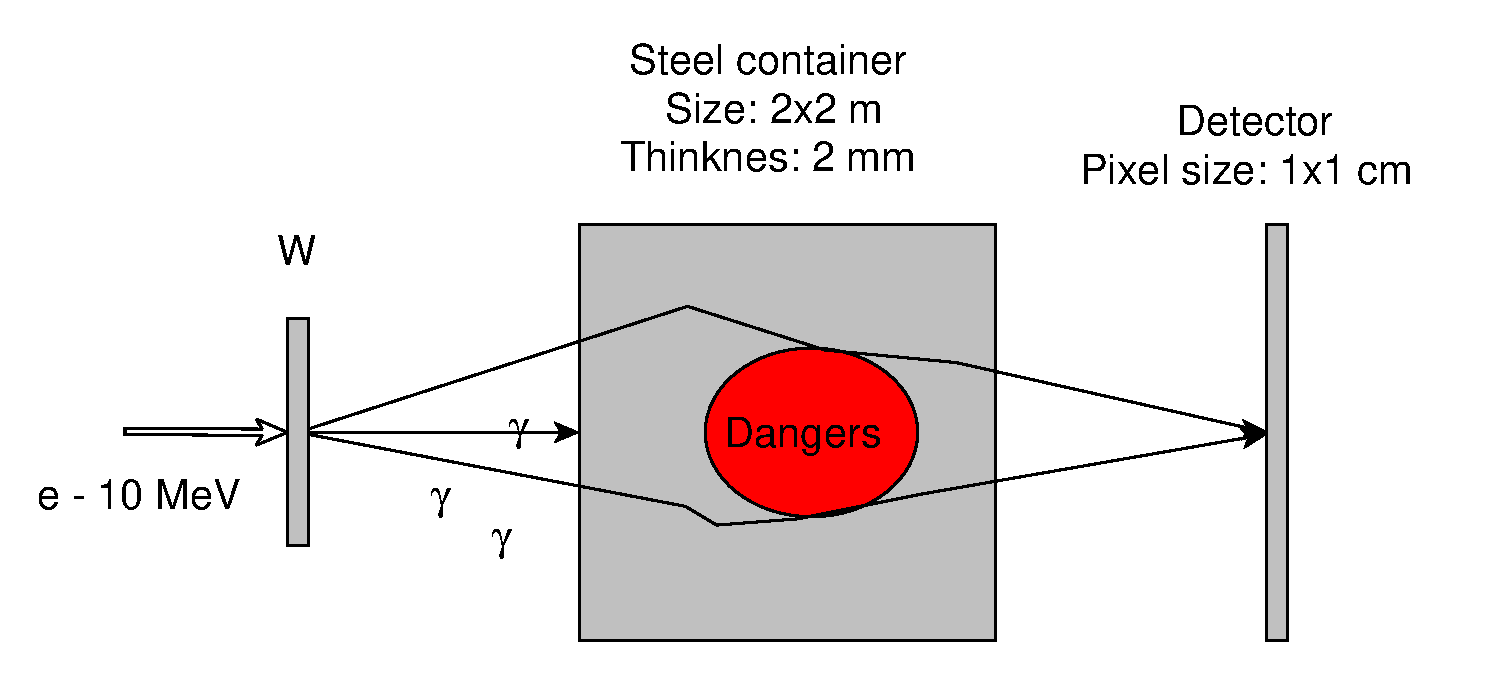
\includegraphics[width=1\textwidth]{figures/yed_schema_1.pdf}
        \end{column}
    \end{columns}  
\end{frame}

\begin{frame}
    \frametitle{Simulation: Preliminary estimates}
    \begin{columns}
        \begin{column}{0.5\textwidth}
            Very dangerous item\\
            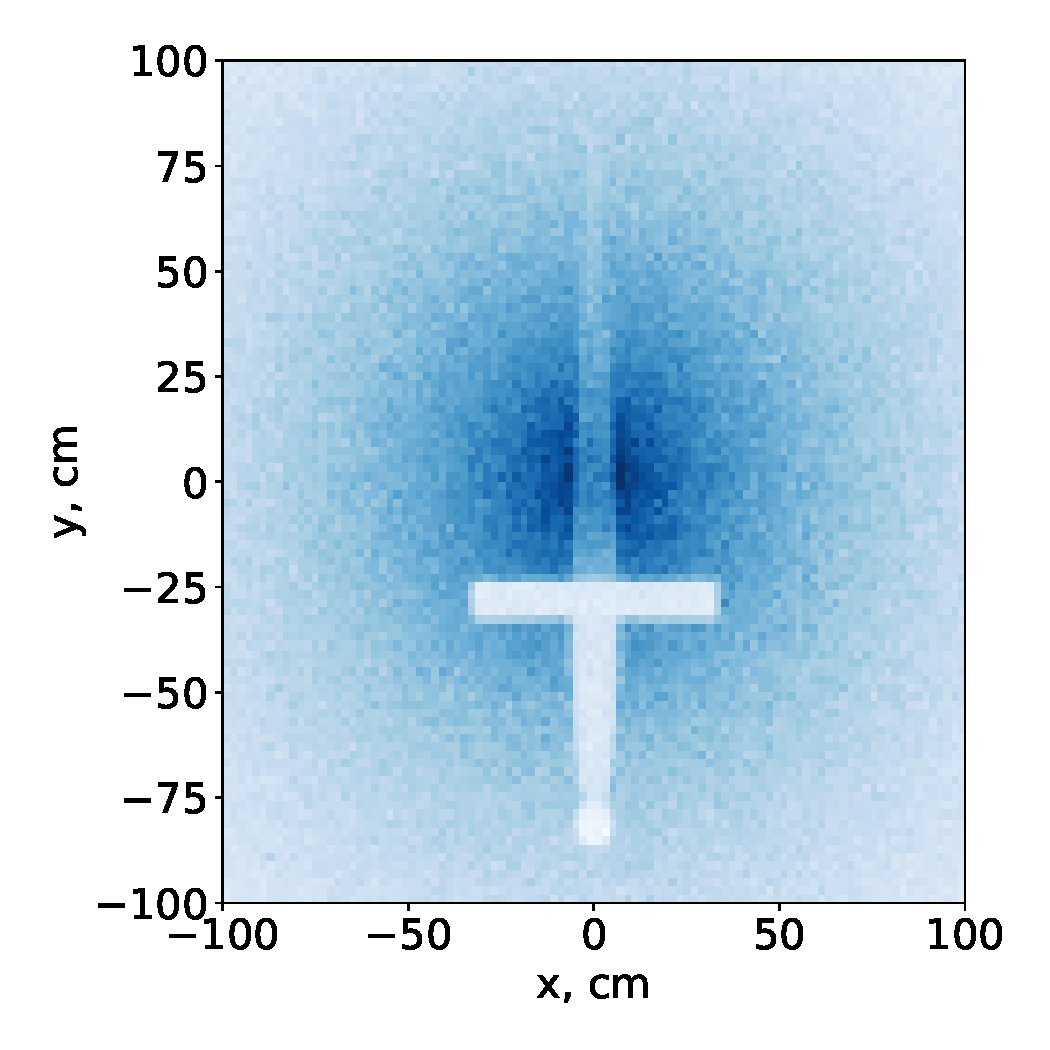
\includegraphics[width=1\textwidth]{figures/Sword.pdf}
        \end{column}
        \begin{column}{0.5\textwidth}
            Uranium cube (6cm) in a lead sphere (thickness -- 1 cm)\\
            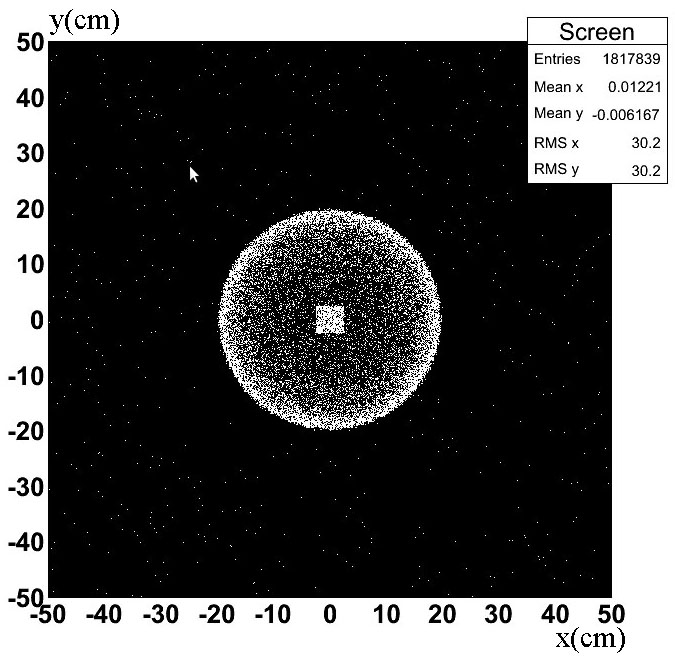
\includegraphics[width=1\textwidth]{figures/sim_cube_in_orb.jpeg}
        \end{column}
    \end{columns}  
\end{frame}

\begin{frame}
    \frametitle{Simulation: Preliminary estimates}
    \begin{columns}
        \begin{column}{0.5\textwidth}
            \centering Search of the explosive\\
            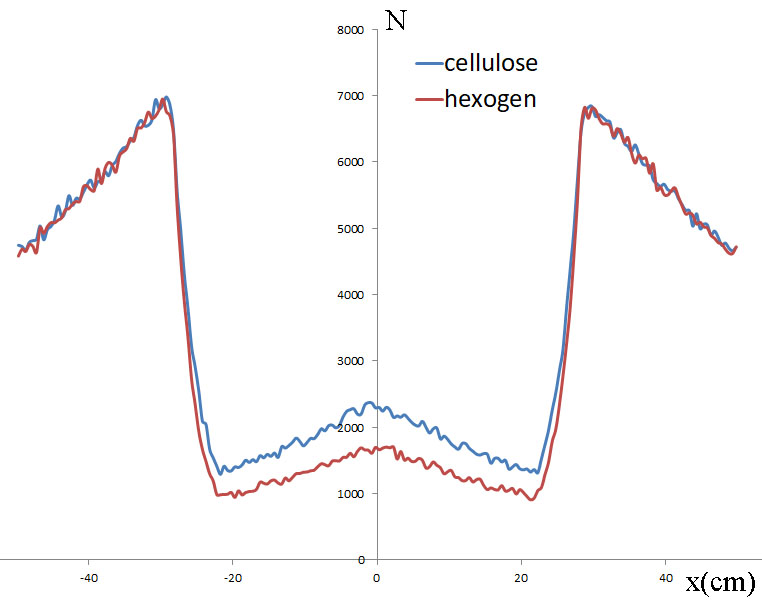
\includegraphics[width=1\textwidth]{figures/sim_hexogen.jpeg}
            
        \end{column}
        \begin{column}{0.5\textwidth}
            Comparison the energy spectrum for aluminium and uranium orb (radius -- 1 cm).\\
            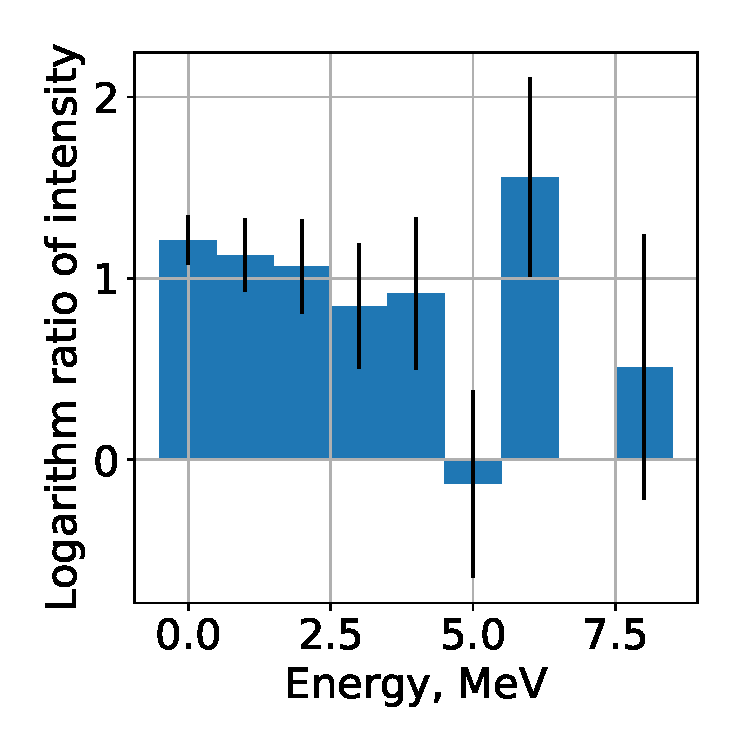
\includegraphics[width=1\textwidth]{figures/Difference.pdf}
        \end{column}
    \end{columns}  
\end{frame}

\begin{frame}
    \frametitle{Simulation: Preliminary estimates}
    \begin{columns}
        \begin{column}{0.5\textwidth}
            The energy deposit in detector cells for several materials\\
            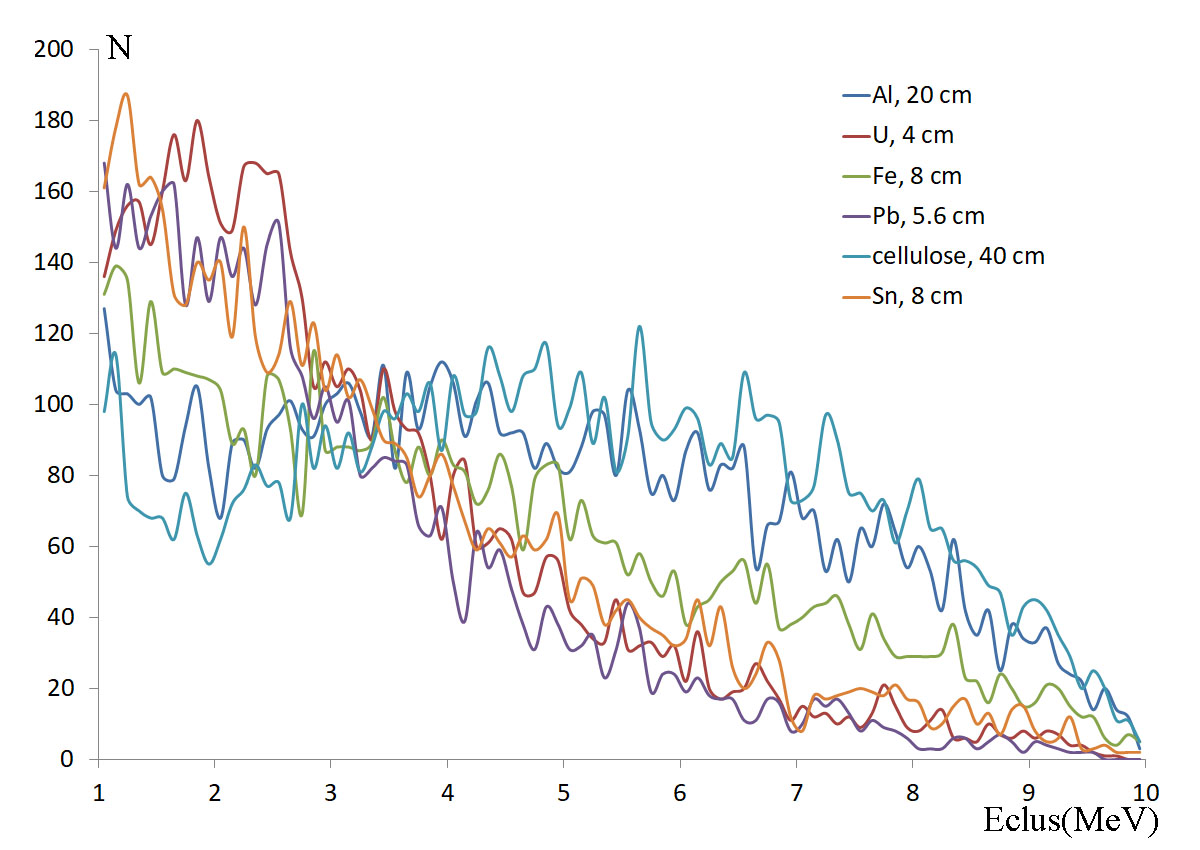
\includegraphics[width=1\textwidth]{figures/sim_1.jpeg}
            
        \end{column}
        \begin{column}{0.5\textwidth}
            N -- number of detector cells
            $$
           \frac{N[E_{dep} < 3~MeV]}
            {N[E_{dep} > 3~MeV]}
            $$
       
            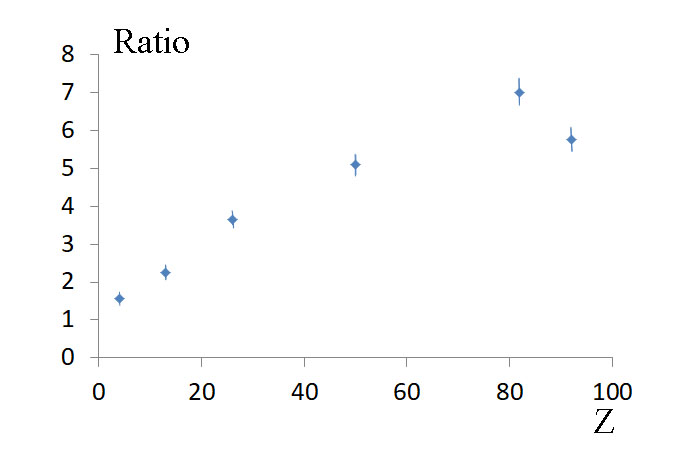
\includegraphics[width=1\textwidth]{figures/sim_2.jpeg}
        \end{column}
    \end{columns}  
\end{frame}
%-------------Моделирование, часть 2 --------------------------
    \begin{frame}
    \frametitle{Simulation: Thickness reconstruction for the 1-D case}
    \begin{columns}
        \begin{column}{0.4\textwidth}
            \begin{block}{Simple model}
                Attenuation of gamma ray flux is defined as:
                                        $$
                \frac{N(E)}{N_0(E)} = \exp(-\sum_i \Sigma^{mean}_i(E)x_i)
                $$
                where $x_i$ --- thickness of the $i$-layer, $\Sigma^{mean}_i$ --- mean cross-section for group of materials, $N,~N_0$ --- the number of gamma.
                \begin{itemize}
                    \item Disregard secondary scattering.
                    \item Disregard the annihilation line.
                \end{itemize}

                   
            \end{block}

        \end{column}
        \begin{column}{0.55\textwidth}
                  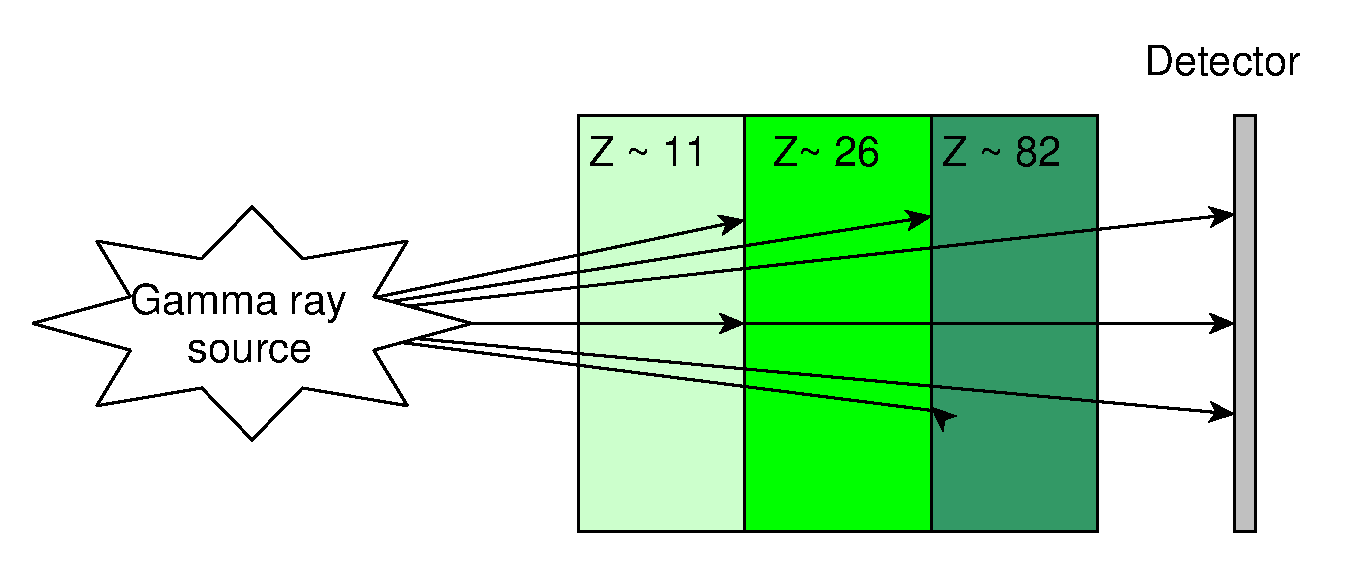
\includegraphics[width=1\textwidth]{figures/yed_schema_2.pdf}
                \begin{block}{Reconstruction algorithm}
                    \begin{itemize}
                        \item Full thickness is known.
                        \item Find thickness using least squares:                  
                        
                    \end{itemize}
                    $$
                    \sum_E(\ln \frac{N(E)}{N_0(E)} + \sum_i \Sigma^{mean}_i(E)x_i))^2 \to min
                    $$
                \end{block}


        \end{column}
    \end{columns}  
\end{frame}

 \begin{frame}
    \frametitle{Thickness reconstruction: Example}
    \begin{columns}
        \begin{column}{0.4\textwidth}
          We consider the object which has 3 layers of aluminium, iron and lead.\\
          The figure shows a contribution of every reconstructed material in summary attenuation. \\
          The table contains the results of reconstruction.
         
        \end{column}
        \begin{column}{0.7\textwidth} 
            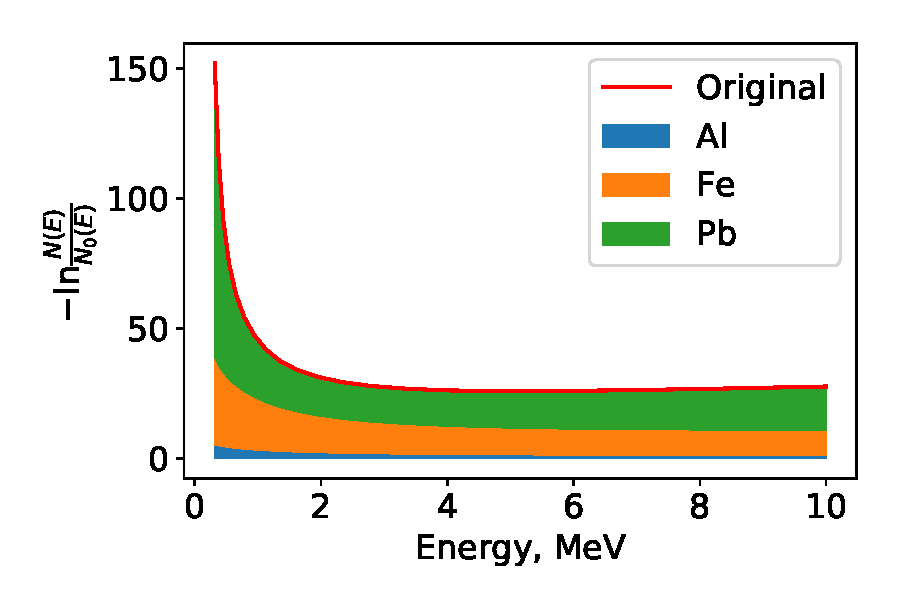
\includegraphics[width=1\textwidth]{figures/reconstruction.pdf}
        \end{column}
    \end{columns}  
\begin{columns}
        \begin{column}{0.5\textwidth}
    
    
    \begin{tabular}[c]{|c|c|c|}
        \hline 
        Material & Real, cm & Reconstructed, cm \\ 
        \hline 
        Al & 20 & 19.6 \\ 
        \hline 
        Fe & 40 & 41.6 \\ 
        \hline 
        Pb & 30 & 28.7 \\ 
        \hline 
    \end{tabular}
    
\end{column}
\end{columns}  
\end{frame}

 \begin{frame}
\frametitle{Simulation: Thickness reconstruction for the 1-D case}
\begin{columns}
            \begin{column}{0.4\textwidth}
                Also we conducted several numeric experiments for different thickness.
                \begin{itemize}
                    \item Aluminium, Iron and Lead are used.
                    \item Several sets of thickness with full thickness from 30 cm to 180 cm.
                    \item The energy grid spacing emulates the detector with  10 \% resolution. 
                    
                \end{itemize}
            \end{column}
    \begin{column}{0.7\textwidth} 
        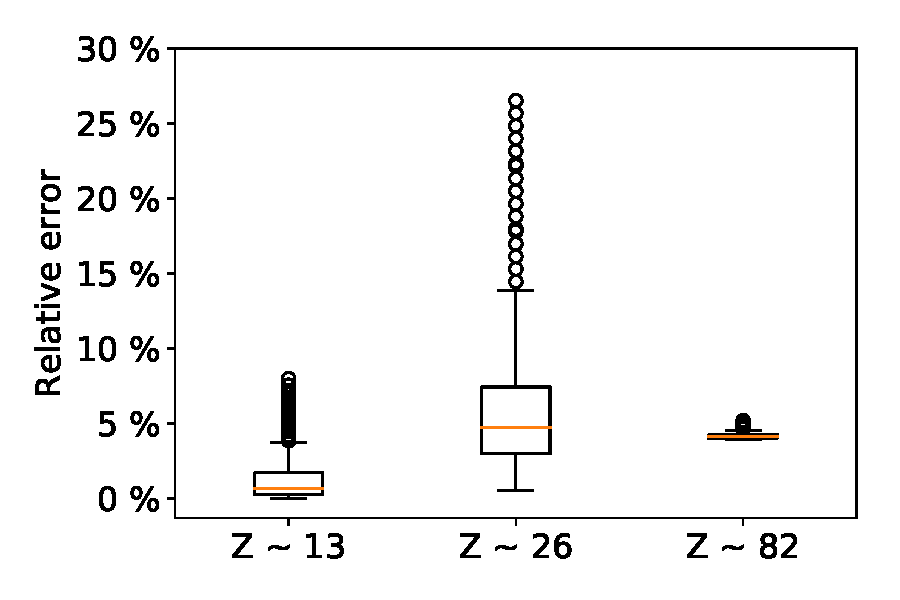
\includegraphics[width=1\textwidth]{figures/relError.pdf}
    \end{column}
\end{columns}  
\end{frame}

    \begin{frame}
        %3d -томография
    \frametitle{Simulation: Perspectives}
    \begin{columns}
                \begin{column}{1\textwidth}
                    \begin{itemize}
                        \item If we use energy-space distribution we can develop the algorithm for the \textbf{3D-tomography} 
                      
                    \end{itemize}

                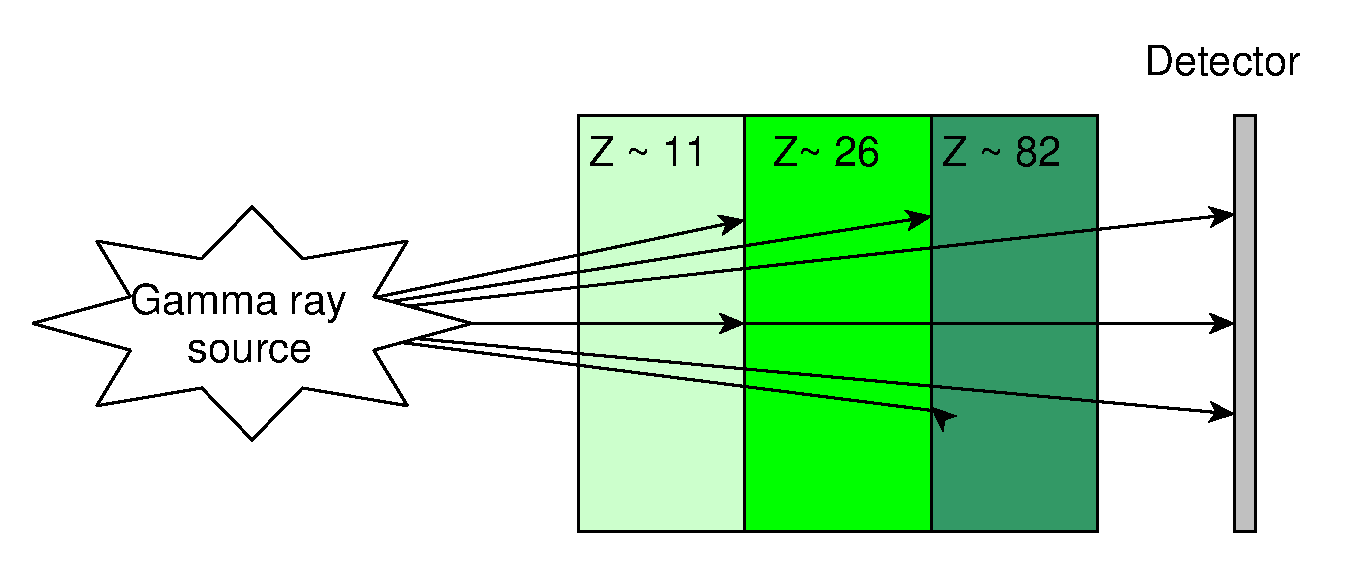
\includegraphics[width=1\textwidth]{figures/yed_schema_2.pdf}
                
            \end{column}
    \end{columns}  
\end{frame}

%-------------Экспериментальная часть--------------------------
\begin{frame}
    \frametitle{Experiment: Energy resolution of the detector}
    \begin{columns}
        \begin{column}{0.5\textwidth}
            
            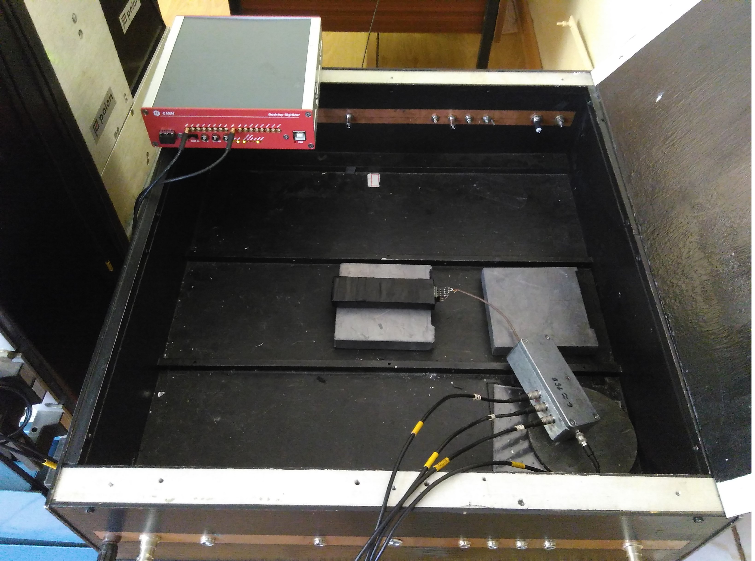
\includegraphics[width=1\textwidth]{figures/setup1.png}\\
            The experiment was conducted by Dr. Guber and Dr. Ivashkin.
        \end{column}
                \begin{column}{0.5\textwidth}
            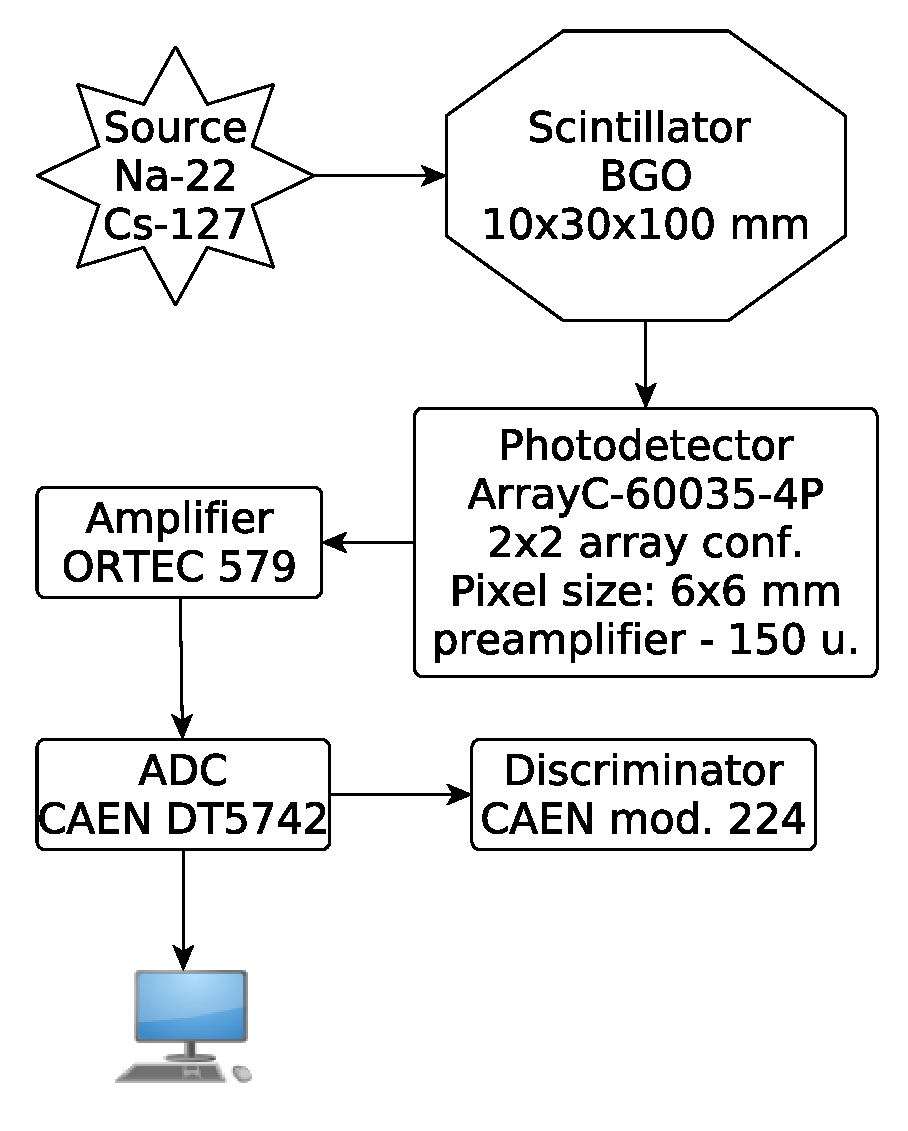
\includegraphics[width=1\textwidth]{figures/yed.pdf}
        \end{column}
    \end{columns}  
\end{frame}

\begin{frame}
    \frametitle{Experiment: Energy resolution of the detector}
    \begin{columns}
        \begin{column}{0.5\textwidth}
            $^{22}Na$ --- $0.511~MeV$\\
            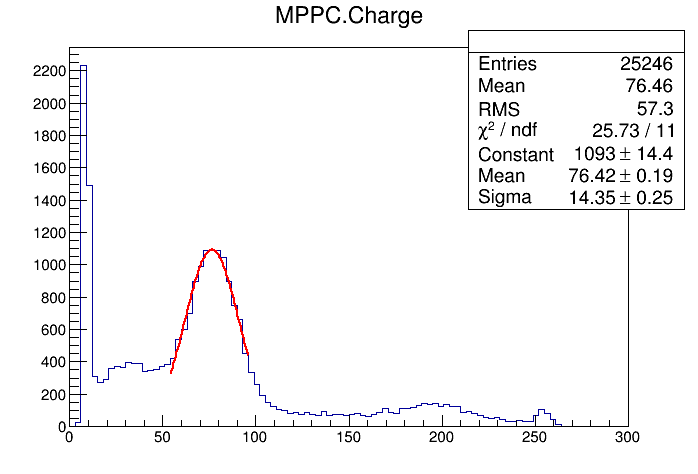
\includegraphics[width=1\textwidth]{figures/setup3.png}
            
        \end{column}
                \begin{column}{0.5\textwidth}
                    $^{22}Na$ --- $1.275~MeV$\\
            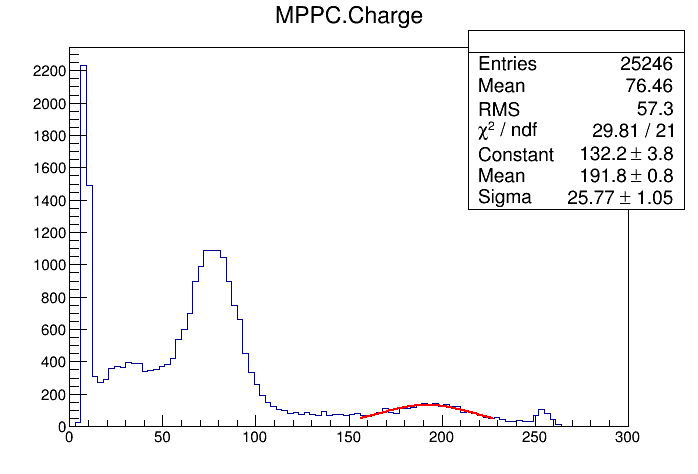
\includegraphics[width=1\textwidth]{figures/setup4.png}
        \end{column}
    \end{columns} 
    
    \begin{columns}
    \begin{column}{0.5\textwidth}
        $^{137}Cs$ --- $0.662~MeV$\\
        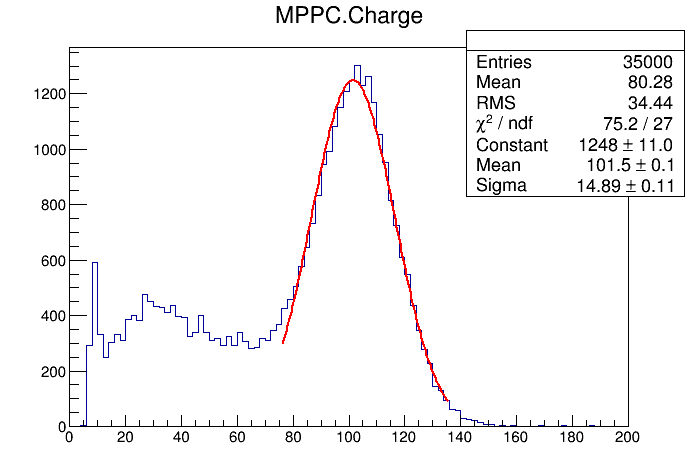
\includegraphics[width=1\textwidth]{figures/setup2.png}
    \end{column}
    \begin{column}{0.5\textwidth}
                The sum of signals from 2 photodiode\\
                Noise threshold: 100 KeV\\
                ~\\
        \begin{tabular}[c]{|c|c|}
             \hline 
            Energy, MeV & Sigma/Mean \\
            \hline 
           0.511 & 14.7\%  \\ 
            \hline 
            0.662 & 19\%\\ 
            \hline 
            1.275 & 13\%\\
            \hline 
        \end{tabular} 
\\

    \end{column}
\end{columns} 
     
\end{frame}

%--------------- Выводы ----------------
\begin{frame}
    \frametitle{Conclusion}
    
    \begin{block}{Results}%<1->   
    \begin{enumerate}
        \item The measurement of the gamma ray spectrum allows to identify cargo belonging to the group of materials with certain $Z_{eff}$.
        \item Also it allows to define the thickness of layers from different elements with the accuracy about 25\%.
        \item The energy resolution of the detector based on a BGO scintillator was studied.  For the photodetector with full array of pixels the energy resolution is expected about 10\%.
    \end{enumerate}
    \end{block}
\begin{block}{Plans and perspectives}%<3->
    With financial support can be developed:
    \begin{enumerate}
        \item The program which checks cargo of a transport container  for compliance cargo manifest
        \item The algorithm for the 3D gamma-tomography.
    \end{enumerate}
\end{block}

\end{frame}

\begin{frame}
    \frametitle{Thank you for your attention}
            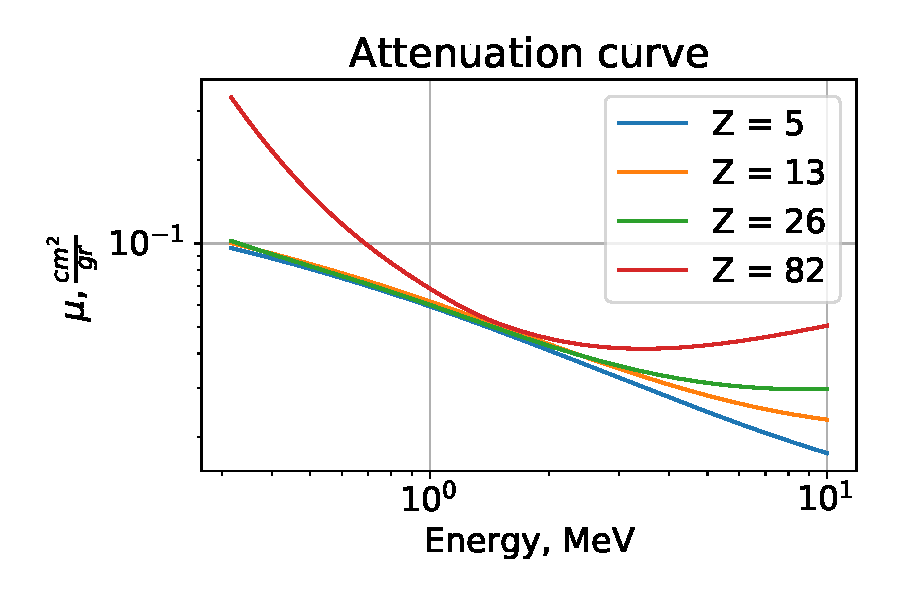
\includegraphics[width=1\textwidth]{figures/Attenuation.pdf}
\end{frame}

\end{document} 
%
%\begin{frame}
%    \frametitle{}
%\end{frame}
